\documentclass[../documentation.tex]{subfiles}
\begin{document}


\subsection{Requirements}

\bgroup{}
\def\arraystretch{1.25}
\begin{center}
    \begin{tabular}{ |l|p{9cm}| }
        \hline
        \multicolumn{2}{|c|}{\textbf{Req-00}} \\
        \hline
        \textbf{Name} & Proof-of-Work \\
        \hline
        \textbf{Priority} & 1 \\
        \hline
        \textbf{Version} & 1.1 \\
        \hline
        \textbf{Notes} & none \\
        \hline
        \textbf{Description} & The blockchain consensus must be based on the Proof-of-Work algorithm. \\
        \hline
    \end{tabular}
\end{center}
\egroup{}

\bgroup{}
\def\arraystretch{1.25}
\begin{center}
    \begin{tabular}{ |l|p{9cm}| }
        \hline
        \multicolumn{2}{|c|}{\textbf{Req-01}} \\
        \hline
        \textbf{Name} & Peer Discovery \\
        \hline
        \textbf{Priority} & 1 \\
        \hline
        \textbf{Version} & 1.1 \\
        \hline
        \textbf{Notes} & none \\
        \hline
        \textbf{Description} & Nodes must be able to find and connect to eachother. \\
        \hline
        \multicolumn{2}{|c|}{\textbf{Subrequirements}} \\
        \hline
        \textbf{Req-01\_0} & Peer discovery based on centralized servers must be minimized. \\
        \hline
    \end{tabular}
\end{center}
\egroup{}

\bgroup{}
\def\arraystretch{1.25}
\begin{center}
    \begin{tabular}{ |l|p{9cm}| }
        \hline
        \multicolumn{2}{|c|}{\textbf{Req-02}} \\
        \hline
        \textbf{Name} & Smart Contract \\
        \hline
        \textbf{Priority} & 1.1 \\
        \hline
        \textbf{Version} & 1.0 \\
        \hline
        \textbf{Notes} & none \\
        \hline
        \textbf{Description} & Nodes must be able to process smart contracts. \\
        \hline
    \end{tabular}
\end{center}
\egroup{}

\bgroup{}
\def\arraystretch{1.25}
\begin{center}
    \begin{tabular}{ |l|p{9cm}| }
        \hline
        \multicolumn{2}{|c|}{\textbf{Req-03}} \\
        \hline
        \textbf{Name} & Programming language \\
        \hline
        \textbf{Priority} & 2 \\
        \hline
        \textbf{Version} & 1.1 \\
        \hline
        \textbf{Notes} & none \\
        \hline
        \textbf{Description} &A custom programming language must be developed in order to write smart contracts. \\
        \hline
    \end{tabular}
\end{center}
\egroup{}

\bgroup{}
\def\arraystretch{1.25}
\begin{center}
    \begin{tabular}{ |l|p{9cm}| }
        \hline
        \multicolumn{2}{|c|}{\textbf{Req-04}} \\
        \hline
        \textbf{Name} & Forger tool \\
        \hline
        \textbf{Priority} & 2 \\
        \hline
        \textbf{Version} & 1.1 \\
        \hline
        \textbf{Notes} & none \\
        \hline
        \textbf{Description} & A utility tool to generate keypairs and sign transactions must be developed. \\
        \hline
        %\multicolumn{2}{|c|}{\textbf{Subrequirements}} \\
        %\hline
        %\textbf{Req-01\_0} & There must be a section on the site dedicated to information about blocks, transactions, gas fees. \\
        %\hline
        %\textbf{Req-01\_1} & There must be a section on the site that allows the user to generate a wallet. \\
        %\hline
        %\textbf{Req-01\_2} & There must be a section on the site that allows the user to carry out and control their transactions. \\
        %\hline
        %\textbf{Req-01\_3} & There must be a section in the site that allows the user to carry out the proof of stake, that is to block a determined quantity of coins in order to be chosen as validator. \\
        %\hline
    \end{tabular}
\end{center}
\egroup{}

\bgroup{}
\def\arraystretch{1.25}
\begin{center}
    \begin{tabular}{ |l|p{9cm}| }
        \hline
        \multicolumn{2}{|c|}{\textbf{Req-05}} \\
        \hline
        \textbf{Name} & API \\
        \hline
        \textbf{Priority} & 1 \\
        \hline
        \textbf{Version} & 1.1 \\
        \hline
        \textbf{Notes} & none \\
        \hline
        \textbf{Description} & A node with HTTP POST routes must be developed. \\
        \hline
        \multicolumn{2}{|c|}{\textbf{Subrequirements}} \\
        \hline
        \textbf{Req-05\_0} & There must be a route to get the latest mined blocks \\
        \hline
        \textbf{Req-05\_1} & There must be a route to get block informations \\
        \hline
        \textbf{Req-05\_2} & There must be a route to get wallet informations \\
        \hline
        \textbf{Req-05\_3} & There must be a route to get all the transaction regarding a wallet \\
        \hline
        \textbf{Req-05\_4} & There must be a route to deploy transactions \\
        \hline
        \textbf{Req-05\_5} & Responses must be in the JSON format \\
        \hline
    \end{tabular}
\end{center}
\egroup{}

\bgroup{}
\def\arraystretch{1.25}
\begin{center}
    \begin{tabular}{ |l|p{9cm}| }
        \hline
        \multicolumn{2}{|c|}{\textbf{Req-06}} \\
        \hline
        \textbf{Name} & Miner \\
        \hline
        \textbf{Priority} & 1 \\
        \hline
        \textbf{Version} & 1.1 \\
        \hline
        \textbf{Notes} & none \\
        \hline
        \textbf{Description} & A node that will solve Proof-of-works must be developed. \\
        \hline
        \multicolumn{2}{|c|}{\textbf{Subrequirements}} \\
        \hline
        \textbf{Req-06\_0} & The number of CPUs used must be configurable \\
        \hline
    \end{tabular}
\end{center}
\egroup{}

\bgroup{}
\def\arraystretch{1.25}
\begin{center}
    \begin{tabular}{ |l|p{9cm}| }
        \hline
        \multicolumn{2}{|c|}{\textbf{Req-07}} \\
        \hline
        \textbf{Name} & Executables \\
        \hline
        \textbf{Priority} & 1 \\
        \hline
        \textbf{Version} & 1.1 \\
        \hline
        \textbf{Notes} & none \\
        \hline
        \textbf{Description} & Every software must be shipped in a single executable. \\
        \hline
        \multicolumn{2}{|c|}{\textbf{Subrequirements}} \\
        \hline
        \textbf{Req-07\_0} & Executable for the seeder software \\
        \hline
        \textbf{Req-07\_1} & Executable for the full-node software \\
        \hline
        \textbf{Req-07\_2} & Executable for the miner-node software \\
        \hline
        \textbf{Req-07\_3} & Executable for the api-node software \\
        \hline
        \textbf{Req-07\_4} & Executable for the webserver \\
        \hline
        \textbf{Req-07\_5} & Executable for the forger software \\
        \hline
        \textbf{Req-07\_6} & Executable for the programming language compiler \\
        \hline
        \textbf{Req-07\_7} & Every executable must have an help page \\
        \hline
    \end{tabular}
\end{center}
\egroup{}

\bgroup{}
\def\arraystretch{1.25}
\begin{center}
    \begin{tabular}{ |l|p{9cm}| }
        \hline
        \multicolumn{2}{|c|}{\textbf{Req-08}} \\
        \hline
        \textbf{Name} & Website \\
        \hline
        \textbf{Priority} & 1 \\
        \hline
        \textbf{Version} & 1.1 \\
        \hline
        \textbf{Notes} & none \\
        \hline
        \textbf{Description} & A website about the blockchain must be developed. \\
        \hline
        \multicolumn{2}{|c|}{\textbf{Subrequirements}} \\
        \hline
        \textbf{Req-08\_0} & The website must contains search form to search blocks, wallets and transaction \\
        \hline
        \textbf{Req-08\_1} & The website must have a section to deploy transactions \\
        \hline
    \end{tabular}
\end{center}
\egroup{}

\pagebreak

\subsection{Planning}

\subsubsection{Initial Gantt Chart}

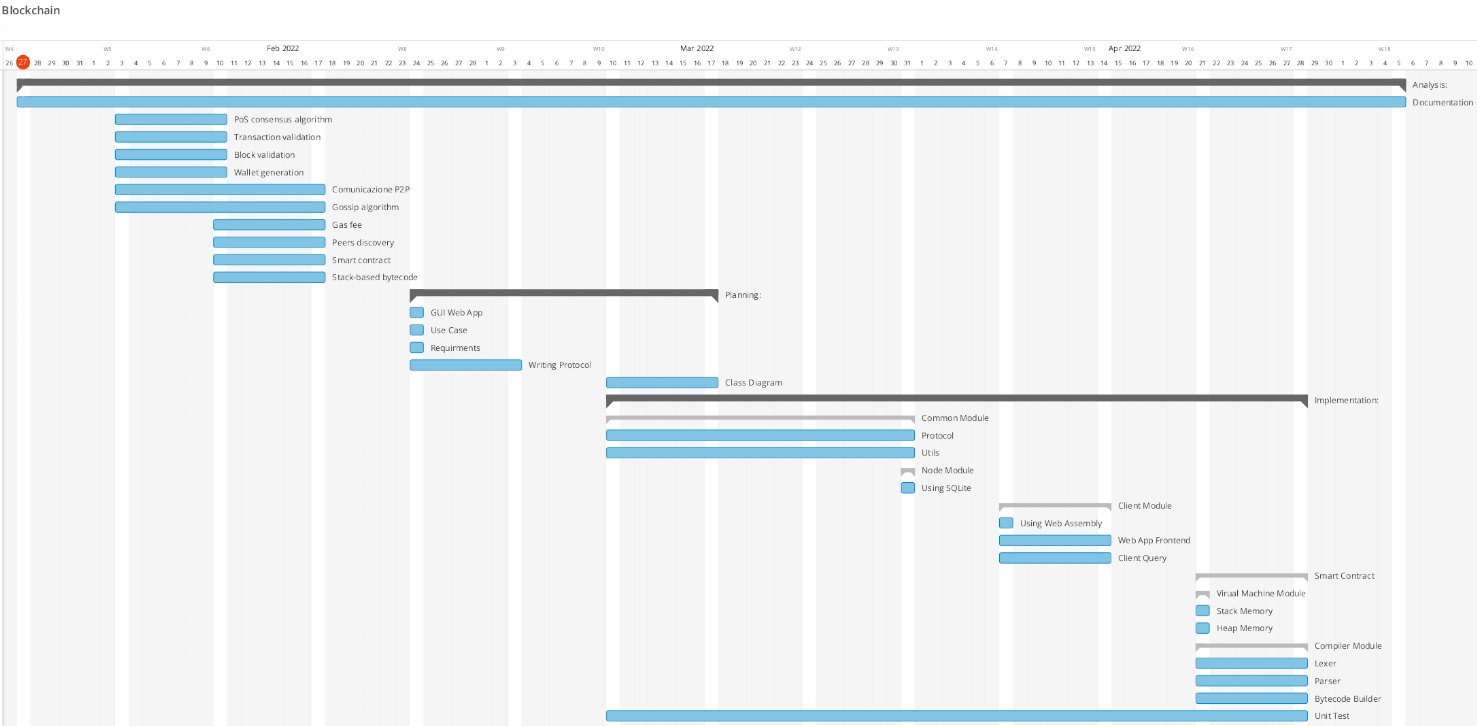
\includegraphics[width=\textwidth]{images/gantt1.png}

\subsubsection{Final Gantt Chart}

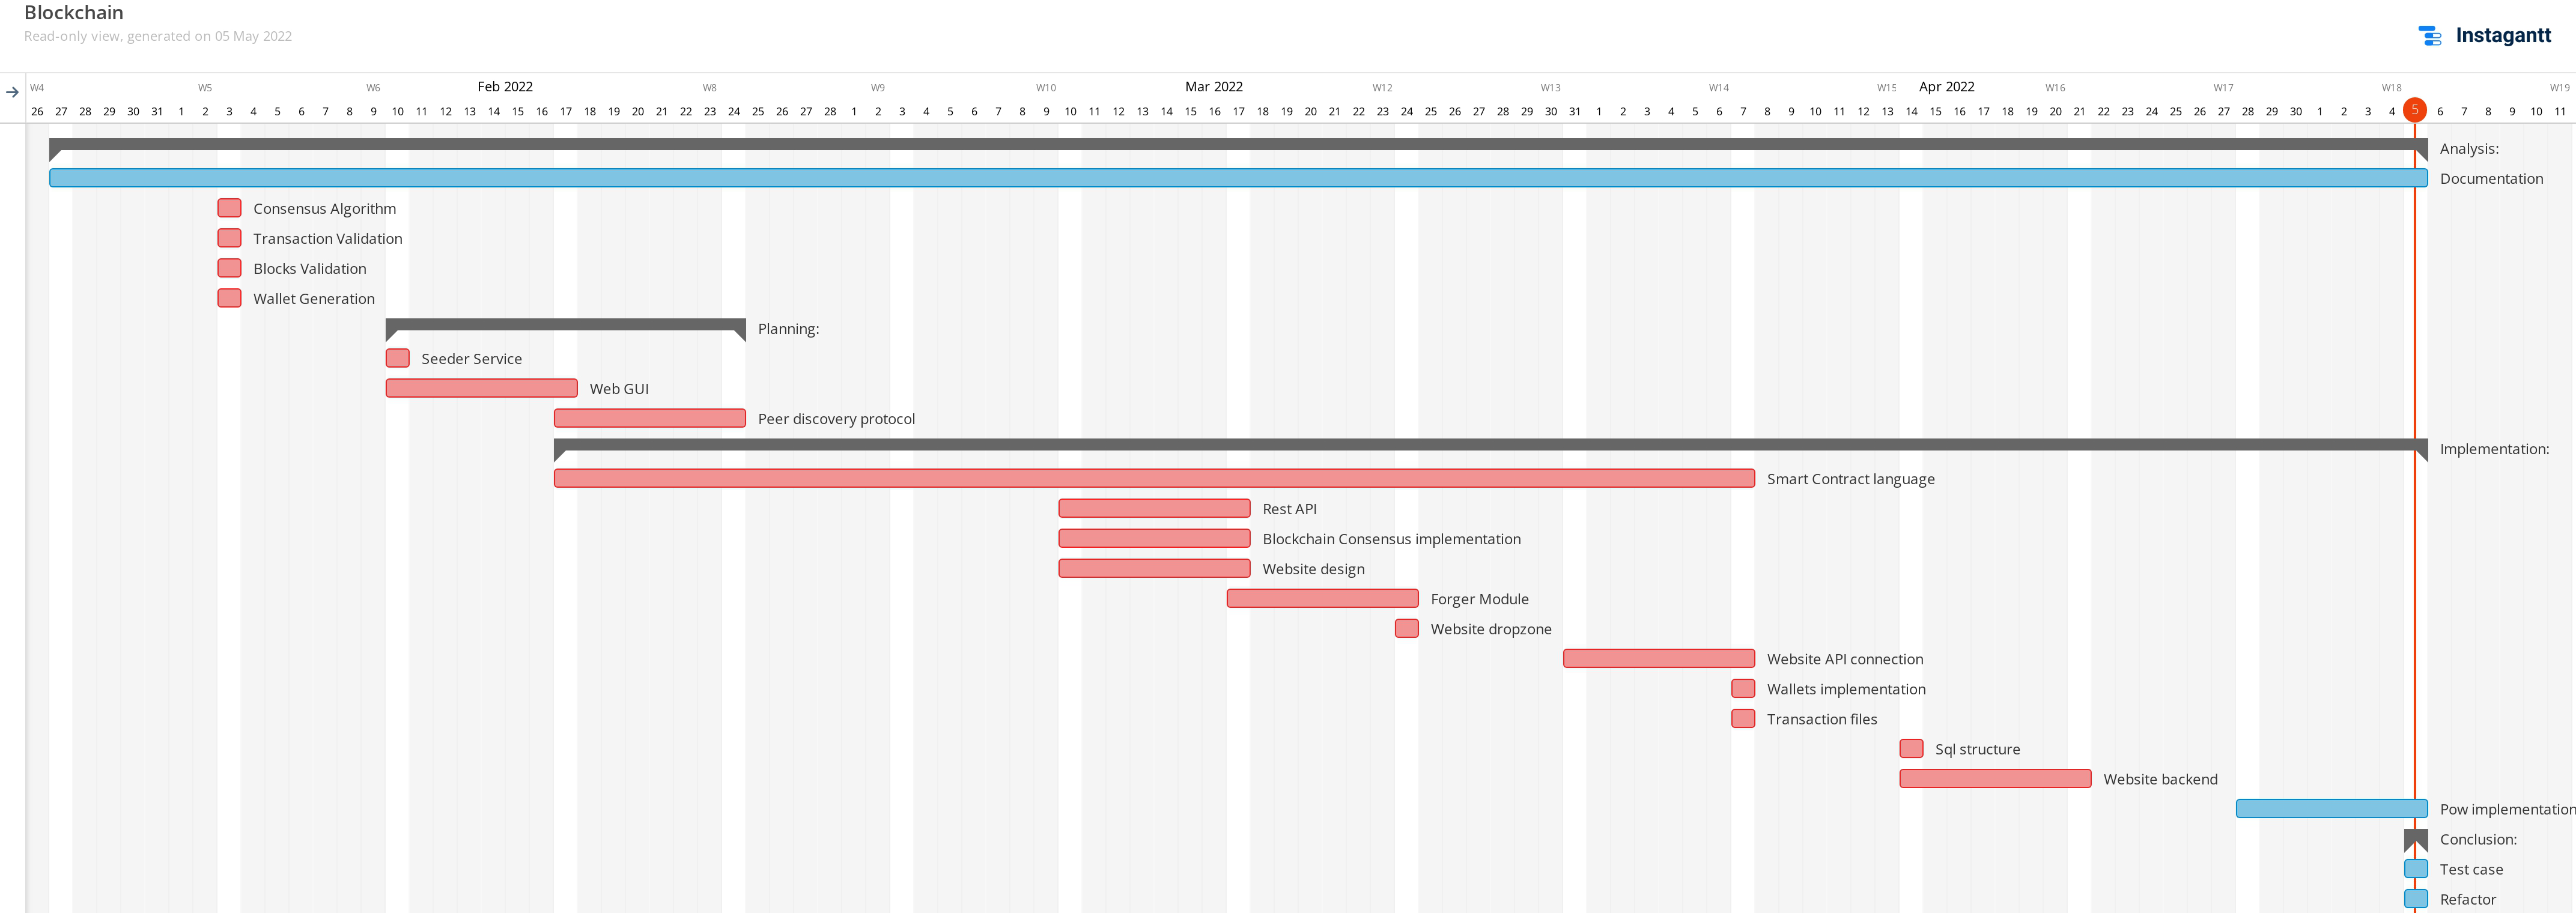
\includegraphics[width=\textwidth]{images/gantt2.png}

\end{document}